\begin{frame}[fragile]{Funktionale Programmierung}
\begin{center}
\Huge
Funktionale Programmierung
\end{center}
\end{frame}

\begin{frame}[fragile]{Warum funktionale Programmierung?}
\begin{itemize}
\onslide+<2->
\item Höhere Abstraktionsmöglichkeiten
\begin{itemize}
\item z. B. Higher Order Functions, Closures
\item ermöglichen knapperen, klareren Code
\end{itemize}

\onslide+<3->
\item Besseres Laufzeitverhalten
\begin{itemize}
\item durch Lazy Evaluation, d. h. Auswertung von Funktionsargumenten erst beim tatsächlichen Zugriff
\end{itemize}

\onslide+<4->
\item Parallelisierung
\begin{itemize}
\item angesichts immer größerer Prozessorzahlen zunehmend wichtiger
\end{itemize}

\onslide+<5->
\item Continuations
\begin{itemize}
\item Beschreibung des Ablaufzustands eines Programms 
\item z. B. zur Live-Migration laufender Prozesse
\end{itemize}

\onslide+<6->
\item Einfache Einbettung domänenspezifischer Sprachen
\begin{itemize}
\item inklusive Typsicherheit
\end{itemize}

\end{itemize}
\end{frame}

% Hinweis: Monaden sind eine Einbettung des imperativen Programmiermodells!

\begin{frame}[fragile]{Und was sind jetzt Monaden?}

Monaden sind
\begin{itemize}
\item eine Abstraktion
\item vereinheitlichen scheinbar verschiedene Aspekte
\item kapseln bestimmte immer wiederkehrende Aspekte
\item helfen so beim Fokussieren
\item schlagen (ganz nebenbei) eine Brücke zwischen der funktionalen und der nichtfunktionalen Welt
\end{itemize}

\end{frame}


\begin{frame}[fragile]{Drei einfache Funktionen}
\begin{lstlisting}
int minus5(int x){ return x - 5; }
	
int mal3(int x){ return x * 3; }
	
int plus7(int x){ return x + 7; }
\end{lstlisting}
\end{frame}

\begin{frame}[fragile]{Drei etwas komplexere Funktionen}
\begin{lstlisting}
Integer minus5(Integer x){ return x - 5; }
	
Integer mal3(Integer x){ return x * 3; }
	
Integer plus7(Integer x){ return x + 7; }
\end{lstlisting}
\end{frame}

\begin{frame}[fragile]{Drei etwas robustere Funktionen}
\begin{lstlisting}
Integer minus5(Integer x){
    if( x == null ) return null;
    return x - 5; 
}
	
Integer mal3(Integer x){ 
    if( x == null ) return null;
    return x * 3; 
}
	
Integer plus7(Integer x){ 
    if( x == null ) return null;
    return x + 7; 
}
\end{lstlisting}
\end{frame}

\begin{frame}[fragile]{Drei Haskell-Funktionen}

Das Haskell-Äquivalent zu Integer:

\begin{lstlisting}
data Maybe a = Just a
             | Nothing
\end{lstlisting}

\onslide+<2->
~

Unsere Funktionen in Haskell:

\begin{lstlisting}
minus5 Nothing  = Nothing
minus5 (Just x) = Just (x - 5)

mal3   Nothing  = Nothing
mal3   (Just x) = Just (3 * x)

plus7  Nothing  = Nothing
plus7  (Just x) = Just (x + 7)
\end{lstlisting}
\end{frame}


%%%%%%%%%%%%%%%%%%%%%%%%%%%%%%%%%%%%%%%%%%%%%%%%%%%%

\begin{frame}[fragile]{}
\begin{center}
\Huge
Funktionen
\end{center}
\end{frame}

\begin{frame}[fragile]{Ist das eine Funktion?}
\begin{lstlisting}
public int random(){

    return new Random().nextInt();
    
}
\end{lstlisting}
\end{frame}

\begin{frame}[fragile]{Oder das?}
\begin{lstlisting}
public int dienstagsBinIchAnders(int input){

    Date rightNow = new Date();

    if(rightNow.getDay() == TUESDAY){
        return 3 * input - 4;
    } else {
        return 17 - input;
    }
}
\end{lstlisting}
\end{frame}

\begin{frame}[fragile]{Oder das?}
\begin{lstlisting}
public int giveNumberAndSaySomething(){

    System.out.println("Hallo Herbstcampus!");
    
    return 7;
}
\end{lstlisting}
\end{frame}


\begin{frame}[fragile]{Oder vielleicht das?}
\begin{lstlisting}
public int throwSomething(int number){
    if( number == 7 ){
        throw new RuntimeException();
    }
    
    return number + 1;
}
\end{lstlisting}
\end{frame}


\begin{frame}[fragile]{Was die Mathematiker darüber denken...}
\onslide+<2->
\begin{minipage}[t]{3.5cm}
\begin{tabular}{|c|c|}
\textbf{x} & \textbf{f( x )}  \\ \hline
1 & 3  \\
3 & 3  \\
7 & 2  \\
12 & 4
\end{tabular} 
\end{minipage} 
\hfill
\onslide+<3->
\begin{minipage}[t]{5.5cm}
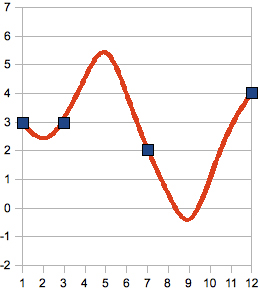
\includegraphics[height=4.5cm]{1Funktion.jpg}
\end{minipage}
~ \\
\onslide+<4->
\begin{eqnarray*}
f(x) &=& \left\{ 
\begin{array}{lll}
3 & & x < 5 \\
2 & wenn & 5 \leq x < 10 \\
4 & & 10 \leq x
\end{array} \right.
\end{eqnarray*}

\end{frame}

%//////////////////////////////////////////////////////////////////////////////////////////////////////////////////////////////////////////////////////////////////////////////////////////////

\begin{frame}[fragile]{Funktionen}
\begin{center}
\Large
Schauen wir nochmal genauer hin...
\end{center}
\end{frame}


\begin{frame}[fragile]{Zufall...}
\begin{lstlisting}
public int random(){

    <R>

}
\end{lstlisting}
\end{frame}

\begin{frame}[fragile]{Abhängigkeit von globalen Daten...}
\begin{lstlisting}
public int dienstagsBinIchAnders(int input){

    <D>

    if(rightNow.getDay() == TUESDAY){
        return 3 * input - 4;
    } else {
        return 17 - input;
    }
}
\end{lstlisting}
\end{frame}

\begin{frame}[fragile]{Textausgaben auf die Konsole...}
\begin{lstlisting}
public int giveNumberAndSaySomething(){

    <P>"Hallo Herbstcampus!"<)>
    
    return 7;
}
\end{lstlisting}
\end{frame}


\begin{frame}[fragile]{Exceptions...}
\begin{lstlisting}
public int throwSomething(int number){
    if( number == 7 ){
        <T>
    }
    
    return number + 1;
}
\end{lstlisting}
\end{frame}

%//////////////////////////////////////////////////////////////////////////////////////////////////////////////////////////////////////////////////////////////////////////////////////////////




\begin{frame}[fragile]{Kann man da denn nix machen?}
\onslide+<2->
Doch!

\vspace{1cm}

\onslide+<3->
Mal angenommen, man könnte die gezeigten Beispiele so verändern, dass sie echte Funktionen würden, bei gleichem Verhalten...

\end{frame}


\begin{frame}[fragile]{Seiteneffekt: String-Ausgabe}
\begin{lstlisting}
public int giveNumberAndSaySomething(){
    System.out.println("Hallo Herbstcampus!");
    return 7;
}
\end{lstlisting}
\end{frame}

\begin{frame}[fragile]{Zusammenfassen von Resultat und Seiteneffekt}
\begin{lstlisting}
public class ResultAndOutput {

    public int result;
    public String output;
	
    public ResultAndOutput(int result, String output) {
        this.result = result;
        this.output = output;
    }
}
\end{lstlisting}
\end{frame}

\begin{frame}[fragile]{Funktion ohne Seiteneffekt}
\begin{lstlisting}
ResultAndOutput giveNumberAndSaySomething_Pure(){
    return new ResultAndOutput(7, "Hallo Herbstcampus!");
}
\end{lstlisting}
\end{frame}

\begin{frame}[fragile]{Noch eine Funktion}
\begin{lstlisting}
int addAndSaySomething(int input){
    System.out.println("Ich kann rechnen!");
    return 3 * input;
}
\end{lstlisting}
\onslide+<2->
Konkatenation:
\begin{lstlisting}
addAndSaySomething( giveNumberAndSaySomething() );
\end{lstlisting}	

\onslide+<3->
Das geht nicht mehr:
\begin{lstlisting}
addAndSaySomething( giveNumberAndSaySomething_Pure() );
\end{lstlisting}	
\end{frame}


\begin{frame}[fragile]{Naiver Lösungsansatz}
\begin{lstlisting}
ResultAndOutput addAndSaySomething_Naiv(ResultAndOutput input){
    return new ResultAndOutput(3 * input.result, 
                input.output + "\n" + "Ich kann rechnen!");
}
\end{lstlisting}

\onslide+<2->
Funktioniert wieder:
\begin{lstlisting}
addAndSaySomething_Naiv( giveNumberAndSaySomething_Pure() );
\end{lstlisting}

\onslide+<3->
Immenser Overhead!
\end{frame}


\begin{frame}[fragile]{Verallgemeinerter Lösungsansatz}
\begin{lstlisting}
ResultAndOutput addAndSaySomething_Pure(int input){
    return new ResultAndOutput(3 * input, "Ich kann rechnen!");
}
\end{lstlisting}

\onslide+<2->
Funktioniert wieder nicht:
\begin{lstlisting}
addAndSaySomething_Pure( giveNumberAndSaySomething_Pure() );
\end{lstlisting}
\end{frame}


\begin{frame}[fragile]{Konkatenierungsfunktion}
\begin{lstlisting}
ResultAndOutput addAndSaySomething_Pure(int input){
    return new ResultAndOutput(3 * input, "Ich kann rechnen!");
}
\end{lstlisting}

\onslide+<2->
Funktioniert wieder nicht:
\begin{lstlisting}
addAndSaySomething_Pure( giveNumberAndSaySomething_Pure() );
\end{lstlisting}
\end{frame}


\begin{frame}[fragile]{Verbinden der Methoden}
In Scala:
\begin{lstlisting}
ResultAndOutput bind(f: int => ResultAndOutput, arg: ResultAndOutput) = {
    val res = f(arg.result)
    return new ResultAndOutput(res.result, arg.output + "\n" + res.output)
  }
\end{lstlisting}
\onslide+<2->
Geht in Java leider nicht!


\onslide+<3->
Dementsprechend in Java auch nicht:
\begin{lstlisting}
bind(addAndSaySomething_Pure , giveNumberAndSaySomething_Pure())
\end{lstlisting}
\end{frame}

\begin{frame}[fragile]{Verbinden der Methoden in Java}
Die zu übergebende Funktion:
\begin{lstlisting}
interface Func {
	ResultAndOutput eval(int arg);
}
\end{lstlisting}

\onslide+<2->
Die bind-Funktion:
\begin{lstlisting}
ResultAndOutput bind(Func f, ResultAndOutput arg) {
    ResultAndOutput res = f.eval(arg.result);
    return new ResultAndOutput(res.result, arg.output + "\n" + res.output);
}
\end{lstlisting}


\onslide+<3->
Jetzt funktioniert es auch in Java:
\begin{lstlisting}
bind(new Func() {
        @Override
        public ResultAndOutput eval(int arg) {
            return addAndSaySomething_Pure(arg);
        }
    }, 
    giveNumberAndSaySomething_Pure());
\end{lstlisting}
\end{frame}

\begin{frame}[fragile]{Alternativen}
In Java auch mit Reflection möglich
\end{frame}

%------

ABER!

Wir wollen sicherstellen, dass die Effekte in der richtigen Reihenfolge ablaufen
- dass sie die richtigen Einflüsse z. B. auf die Ablaufsteuerung haben
- dass alle Effekte erzeugt werden
- dass die Effekte in der Schnittstelle der Funktion sichtbar sind
- dass  dieses Paket an Funktionen von anderen Funktionen entkoppelt ist (parallelisierbar, Ausführungsreihenfolge beliebig)


Außerdem:

- die Behandlung der Effekte soll ausgelagert sein



früher: explizite Fehlerbehandlung (return 0 bzw. <> 0, jeweils explizite Prüfung und Propagation)
heute: es gibt ein implizites Modell, nämlich Exceptions
Zukunft: Wir wollen viele solche Modelle nebeneinander haben können
wir wollen die Modelle auch mischen können


%\begin{frame}[fragile]{Gibt es denn gar keine Gemeinsamkeiten?}
%\onslide+<2->
%Doch!
%
%\begin{itemize}
%\onslide+<3->
%\item Definitionsmenge bzw. die Elemente der Typen der Argumente
%\item Zielmenge bzw. die Elemente des Rückgabetyps
%\onslide+<4->
%\item Konkatenation: $(f \o g)(x) = f(g(x))$ bzw. \textrm{weekdayResult(random())}
%\end{itemize}
%\end{frame}



%%%%%%%%%%%%%%%%%%%%%%%%%%%%%%%%%%%%%%%%%%%%%%%%%%
%\begin{frame}[fragile]{title}
%contents
%%\begin{lstlisting}
%%\end{lstlisting}
%
%%\begin{minipage}{.8 \paperwidth}
%%\includegraphics[width=\textwidth]{OldStateHouse.png} \newline
%%{\tiny \url{http://www.flickr.com/photos/bostonlandmarkscommission/} \hfill \url{http://www.flickr.com/photos/josepha/}}
%%\end{minipage}
%\end{frame}

%%%%%%%%%%%%%%%%%%%%%%%%%%%%%%%%%%%%%%%%%%%%%%%%%%
%\begin{frame}[fragile]{title}
%contents
%%\begin{itemize}
%%\item 
%%\begin{itemize}
%%\item 
%%\end{itemize}
%%\end{itemize}
%
%\end{frame}


%%%%%%%%%%%%%%%%%%%%%%%%%%%%%%%%%%%%%%%%%%%%%%%%%%
{
\usebackgroundtemplate{
\includegraphics[width=\paperwidth,height=\paperheight]{background-slide.png}}
\begin{frame}{Vielen Dank!}

        Code \& Folien auf GitHub:
        \begin{center}
                \url{https://github.com/NicoleRauch/Monaden}
        \end{center}

        \begin{block}{Nicole Rauch}
        \begin{description}[Twitterxx]
                \item[E-Mail]  \href{mailto:nicole.rauch@msg-gillardon.de}{\texttt{nicole.rauch@msg-gillardon.de}}
                \item[Twitter] \href{http://twitter.com/NicoleRauch}{\texttt{@NicoleRauch}}
        \end{description}
        \end{block}
\end{frame}
}
